\documentclass[a4paper,12pt]{article}
\usepackage{graphicx}
\usepackage{amsmath}
\usepackage{hyperref}
\usepackage{amsfonts}
\usepackage{geometry}
\usepackage{float}

\geometry{a4paper, margin=1in}

\renewcommand{\figurename}{Slika}

\title{Prepoznavanje registrskih tablic z uporabo strojnega učenja}
\author{Miha Štih (89221324), Luka Uršič (89221145)}
\date{}

\begin{document}

\maketitle

\section*{Repozitorij projekta}
\url{https://github.com/urluur/Registration-Plate-Recognition}

\section*{Cilj projekta}
Cilj najinega projekta je bil razviti sistem za prepoznavanje in identifikacijo avtomobilskih tablic iz slik. Program naj bi ob podani sliki vrnil registrsko številko in označil lokacijo tablice na sliki, če bi bila ta uspešno prepoznana.

\section*{Izvedba projekta}
Najprej sva začela z izbiro podatkovnega nabora (dataset), ki ga bova uporabila za projekt. Izbrala sva dataset \textit{"Car License Plate Detection"} s spletne strani Kaggle. Kasneje se je izkazalo, da to ni bila najbolj optimalna izbira, saj dataset vsebuje le 433 slik avtomobilov, kar je premalo za učinkovito učenje najinega modela.

Ker so bile slike v datasetu ločene od podatkov, sva se lotila zbiranja teh podatkov. S tem namenom sva pripravila datoteko \texttt{utils.py}, ki vsebuje tri različne funkcije za ekstrakcijo podatkov, saj so bili relevantni podatki podani v XML datotekah za vsako izmed slik posebej. Tako pridobiva podatke \texttt{bbox} iz XML datotek, natančneje \texttt{xmin}, \texttt{xmax}, \texttt{ymin} in \texttt{ymax}, ki določajo kote pravokotnika avtomobilske tablice na sliki. Za pretvorbo slik v uporabne podatke sva uporabila \texttt{numpy}.

\subsection*{Uporaba OpenCV in Pytesseract}
Ko so funkcije za pridobivanje podatkov delovale, sva poskusila uporabiti OpenCV orodje za manipulacijo s slikami. Naučila sva se, kako brati slike, risati pravokotnike in kako zapisati številke tablice kot tekst na sliko. Poskusila sva uporabiti tudi knjižnico \texttt{pytesseract}, ki uporablja Googlov Tesseract OCR Engine za branje teksta s slik, in jo uporabljala skoraj do končne različice projekta.

\pagebreak

\subsection*{Delitev podatkov in učenje modela}
Nato sva uporabila funkcijo \texttt{train\_test\_split} iz knjižnice \texttt{scikit-learn} za naključni razrez podatkov na učno in testno množico. Za velikost testnega seta sva izbrala 15\% vseh podatkov, saj je bil izbran dataset že tako ali tako majhen, tako da nama je ostalo čim več podatkov za učenje modela.

\subsection*{Model in transformacija slik}
Najin naslednji korak je bil sestaviti in naučiti model na izbranem datasetu. Za to sva uporabila \texttt{keras}, saj je preprost za uporabo. Kot model sva izbrala najpreprostejšo verzijo \texttt{Sequential} in dodala nekaj slojev. Najin model je zasnovan tako, da poskuša napovedati lokacije pravokotnika, kjer naj bi bila avtomobilska tablica (lokacijo na sliki). Začela sva tako, da sva slike transformirala na velikost 224x224px in model učila z naslednjimi sloji.

\begin{figure}[H]
    \centering
    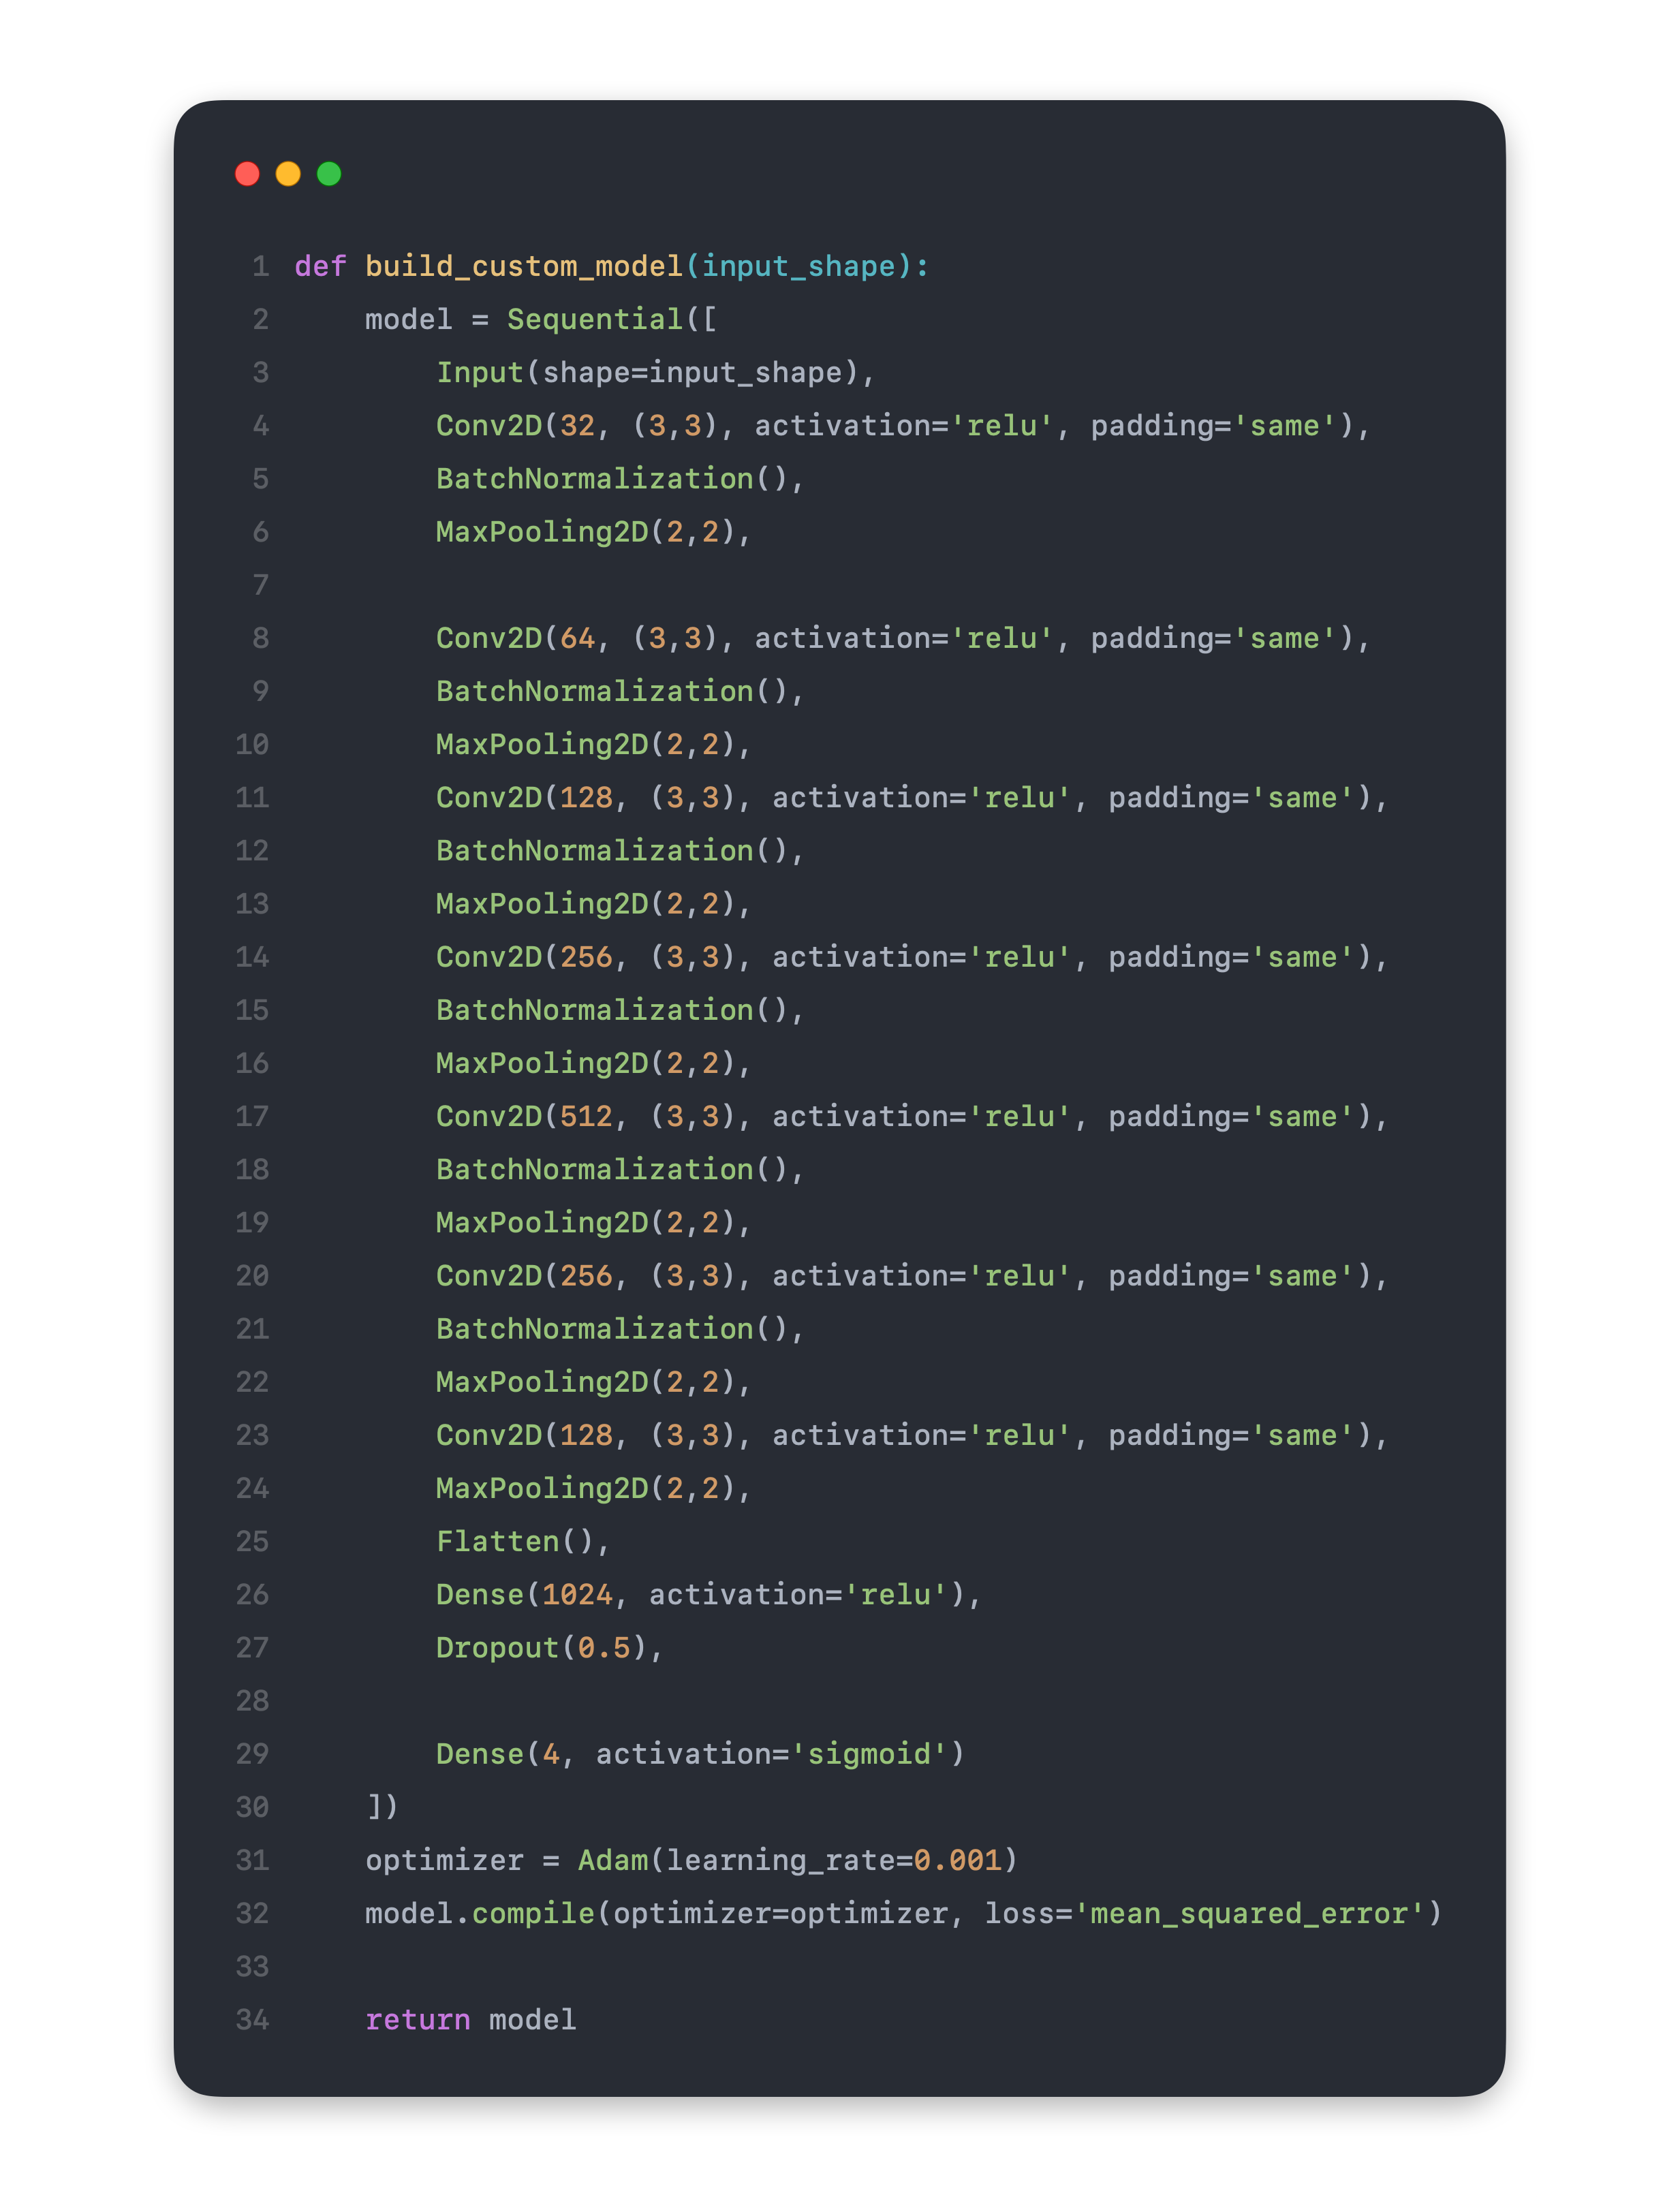
\includegraphics[width=0.75\textwidth]{img/build_custom_model1.png}
    \caption{Začetna sestava modela}
\end{figure}

\subsection*{Izboljšave modela}
Ker model ni dajal želenih rezultatov, sva poskusila več različnih kombinacij slojev in \texttt{loss} funkcij, kot nama je priporočil asistent. Izkazalo se je, da \texttt{mean\_squared\_error} še vedno daje najboljše rezultate. Poskusila sva še \texttt{IoULoss} in \texttt{GIoULoss}, vendar nobena ni presegla učinkovitosti \texttt{mean\_squared\_error}.

Struktura slojev se je medtem spremenila v naslednje:

\begin{figure}[H]
    \centering
    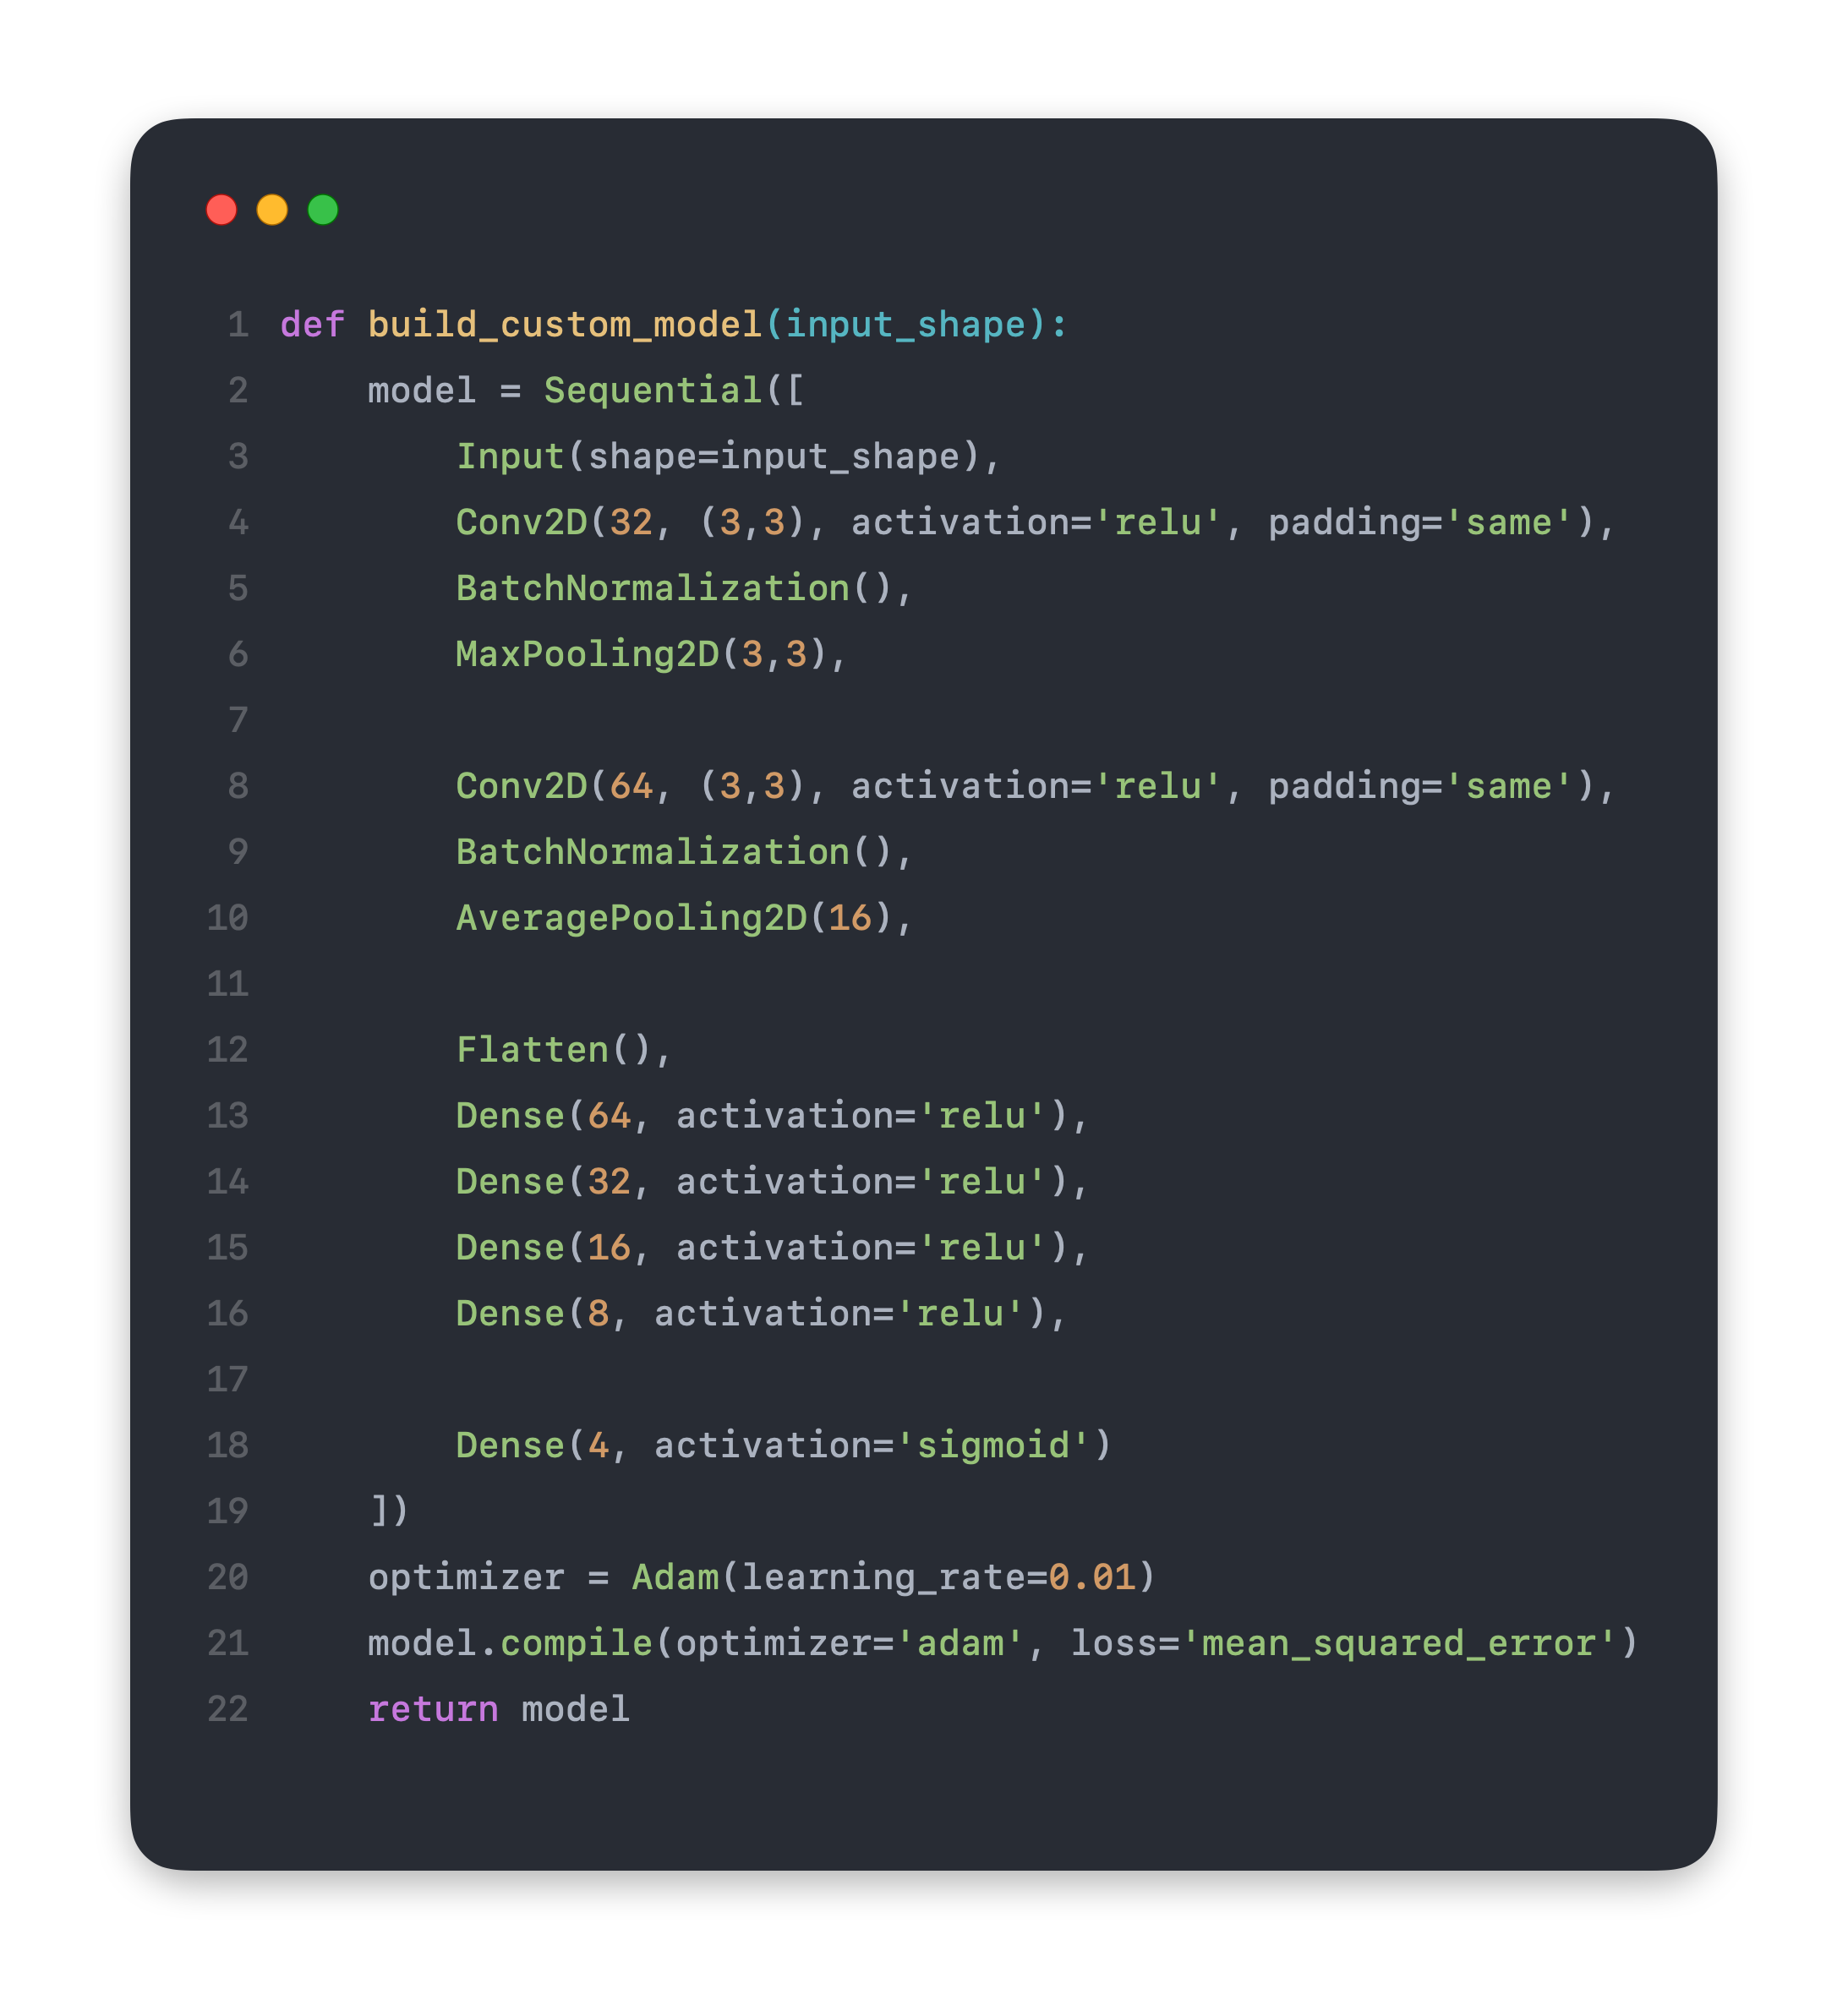
\includegraphics[width=0.8\textwidth]{img/build_custom_model2.png}
    \caption{Končna sestava modela}
\end{figure}

Za boljše učenje sva tudi spremenila velikost slik, ki jih uporabljava za učenje, in sicer iz 224x224px na 500x500px, kar meniva, da je malce pomagalo.

Med optimizacijo slojev sva napisala še funkcijo \texttt{load\_and\_predict}. Deluje tako, da najprej pretvori podano sliko na pravilno velikost, torej 500x500px, nato pa z uporabo modela poskuša najti lokacijo avtomobilske tablice. Ko lokacijo oziroma pravokotnik najde, sliko pretvori v črno-belo in uporabi \texttt{pytesseract} OCR za prepoznavo znakov na tem delu slike. Za vsak slučaj sva dodala še nekaj manevrskega prostora, tako da se prebere slika, ki je na vsako stran za 10px večja od pravokotnika.

Po nekaj preizkusih modela sva na primeru dobila naslednji rezultat:

\begin{figure}[H]
    \centering
    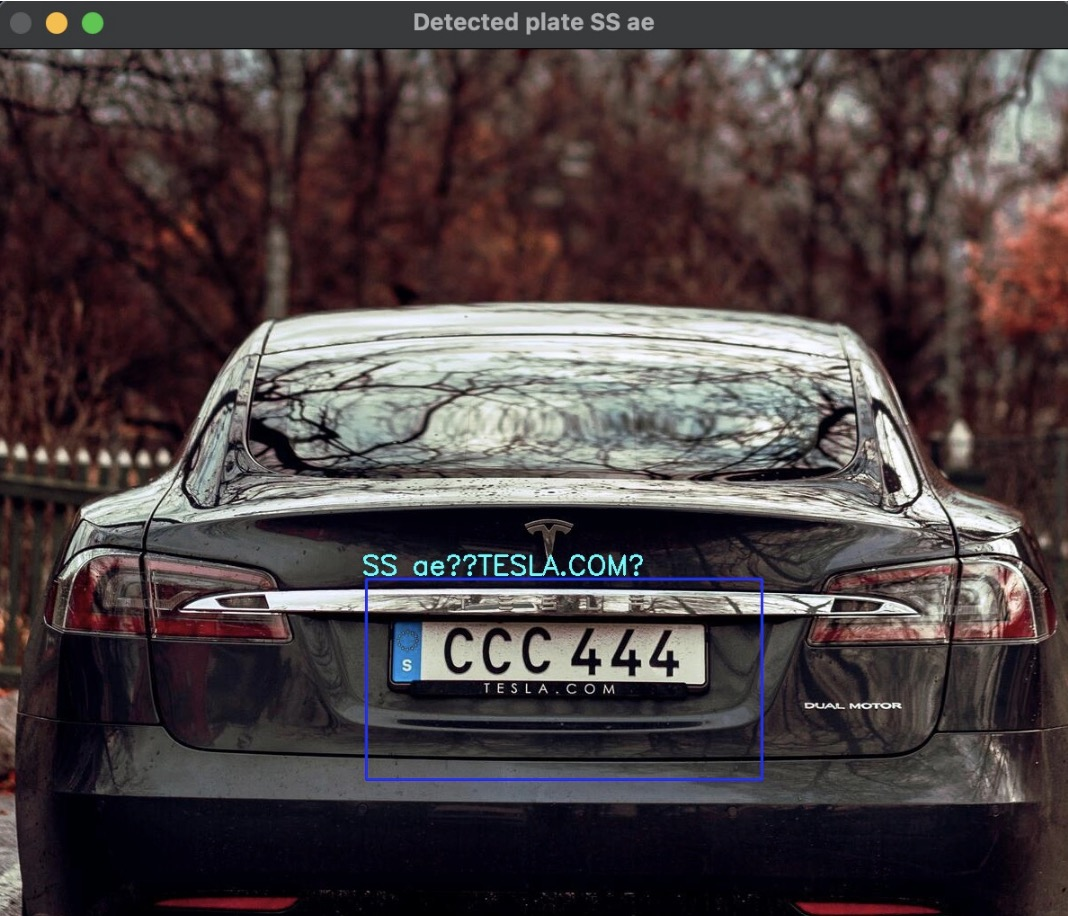
\includegraphics[width=0.6\textwidth]{img/plate_detection1.jpg}
    \caption{Začetna zaznava tablice}
\end{figure}

Kar nama je pokazalo, da prepoznavanje lokacije tablic vsaj približno deluje, medtem ko OCR ne deluje tako, kot bi moral. Ker OCR ni deloval po pričakovanjih, sva se odločila, da ga raje zamenjava z EasyOCR, ki se je izkazal za dosti bolj učinkovitega in sedaj bere tablice tako, kot bi moral. To je razvidno na spodnji sliki (v primerjavi s prejšnjo sliko).

\begin{figure}[H]
    \centering
    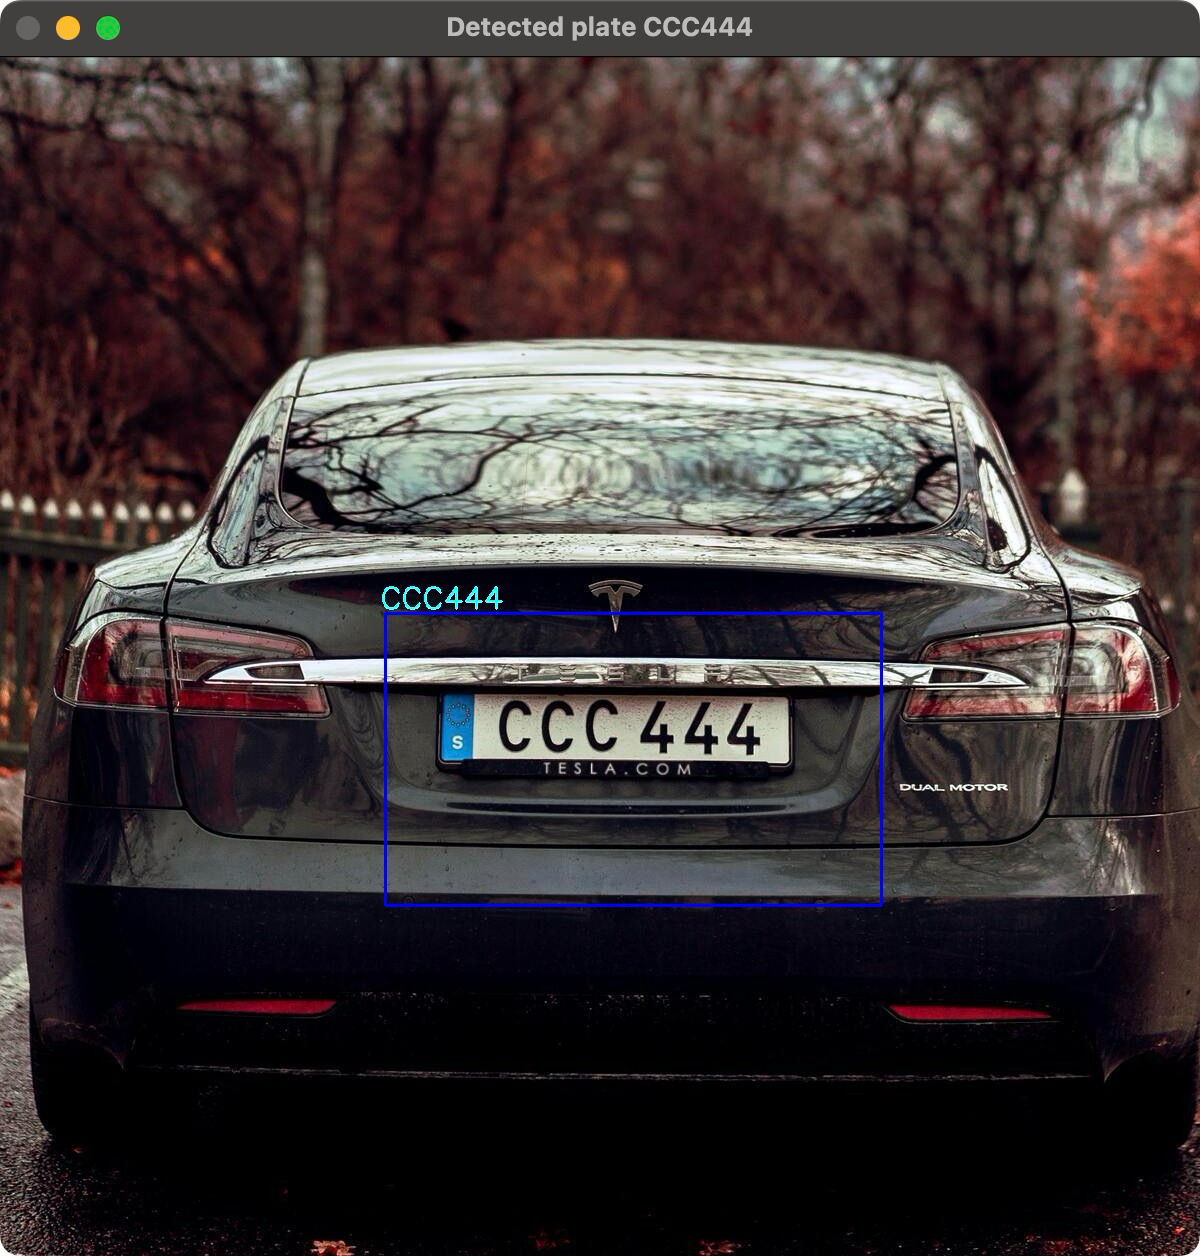
\includegraphics[width=0.6\textwidth]{img/plate_detection2.jpg}
    \caption{Končna zaznava tablice}
\end{figure}

\section*{Nadgradnje}

Ker je na tej točki projekt deloval kot bi moral, sva ga premaknila iz običajnih Python datotek v Jupyter Notebook, da bo lažje za uporabo in nadgradnjo.

Kot dodatno izboljšavo sva uporabila tudi knjižnici \texttt{scikit-learn} in \texttt{matplotlib} za lepšo vizualizacijo delovanja najinega modela. Prikazani so Confusion Matrix, graf napačno pozitivnih primerov v primerjavi s pravilnimi ter graf točnosti.

Za konec je Luka že začel s prvo dejansko nadgradnjo, ki omogoča, da programu ni treba podati slike avtomobila, saj lahko z uporabo kamere tablice bere v realnem času.

\section*{Zaključek}
Projekt naju je presenetil, saj se je izkazal za težjega, kot sva pričakovala. Ker še vedno ne deluje optimalno, meniva, da obstaja nekaj možnih izboljšav. Poudarek bi dala na zamenjavo podatkovnega nabora, kot nama je svetoval že asistent. Trenutno uporabljen dataset je premajhen, da bi se model učinkovito naučil iskati lokacije tablic na slikah, zato bi bil večji dataset več kot dobrodošel.

Poleg tega vidiva še druge možne izboljšave in nadgradnje projekta, saj ima ta potencialno veliko praktično uporabnost na več različnih področjih, vse od nadzora prometa do parkirišč in radarjev.

\section*{Povezave/viri}
\begin{itemize}
    \item \href{https://www.kaggle.com/datasets/andrewmvd/car-plate-detection}{Uporabljen dataset}
    \item \href{https://opencv.org/}{OpenCV}
    \item \href{https://pypi.org/project/pytesseract/}{Pytesseract}
    \item \href{https://keras.io/api/keras\_cv/losses/}{Keras losses}
    \item \href{https://scikit-learn.org/stable/modules/generated/sklearn.model\_selection.train\_test\_split.html}{Train\_test\_split funkcija}
    \item \href{https://numpy.org/}{Numpy}
    \item \href{https://github.com/JaidedAI/EasyOCR}{EasyOCR}
    \item \href{https://matplotlib.org/}{MatPlotLib}
    \item \href{https://www.datacamp.com/tutorial/python-xml-elementtree}{XML parsing}
\end{itemize}

\end{document}
